\documentclass[a4paper, 14pt]{extarticle}

% Поля
%--------------------------------------
\usepackage{geometry}
\geometry{a4paper,tmargin=2cm,bmargin=2cm,lmargin=3cm,rmargin=1cm}
%--------------------------------------


%Russian-specific packages
%--------------------------------------
\usepackage[T2A]{fontenc}
\usepackage[utf8]{inputenc} 
\usepackage[english, main=russian]{babel}
%--------------------------------------

\usepackage{textcomp}

% Красная строка
%--------------------------------------
\usepackage{indentfirst}               
%--------------------------------------             


%Graphics
%--------------------------------------
\usepackage{graphicx}
\graphicspath{ {./images/} }
\usepackage{wrapfig}
%--------------------------------------

% Полуторный интервал
%--------------------------------------
\linespread{1.3}                    
%--------------------------------------

%Выравнивание и переносы
%--------------------------------------
% Избавляемся от переполнений
\sloppy
% Запрещаем разрыв страницы после первой строки абзаца
\clubpenalty=10000
% Запрещаем разрыв страницы после последней строки абзаца
\widowpenalty=10000
%--------------------------------------

%Списки
\usepackage{enumitem}

%Подписи
\usepackage{caption} 

%Гиперссылки
\usepackage{hyperref}

\hypersetup {
	unicode=true
}

%Рисунки
%--------------------------------------
\DeclareCaptionLabelSeparator*{emdash}{~--- }
\captionsetup[figure]{labelsep=emdash,font=onehalfspacing,position=bottom}
%--------------------------------------

\usepackage{tempora}

%Листинги
%--------------------------------------
\usepackage{listings}
\lstset{
  basicstyle=\ttfamily\footnotesize, 
  %basicstyle=\footnotesize\AnkaCoder,        % the size of the fonts that are used for the code
  breakatwhitespace=false,         % sets if automatic breaks shoulbd only happen at whitespace
  breaklines=true,                 % sets automatic line breaking
  captionpos=t,                    % sets the caption-position to bottom
  inputencoding=utf8,
  frame=single,                    % adds a frame around the code
  keepspaces=true,                 % keeps spaces in text, useful for keeping indentation of code (possibly needs columns=flexible)
  keywordstyle=\bf,       % keyword style
  numbers=left,                    % where to put the line-numbers; possible values are (none, left, right)
  numbersep=5pt,                   % how far the line-numbers are from the code
  xleftmargin=25pt,
  xrightmargin=25pt,
  showspaces=false,                % show spaces everywhere adding particular underscores; it overrides 'showstringspaces'
  showstringspaces=false,          % underline spaces within strings only
  showtabs=false,                  % show tabs within strings adding particular underscores
  stepnumber=1,                    % the step between two line-numbers. If it's 1, each line will be numbered
  tabsize=2,                       % sets default tabsize to 8 spaces
  title=\lstname                   % show the filename of files included with \lstinputlisting; also try caption instead of title
}
%--------------------------------------

%%% Математические пакеты %%%
%--------------------------------------
\usepackage{amsthm,amsfonts,amsmath,amssymb,amscd}  % Математические дополнения от AMS
\usepackage{mathtools}                              % Добавляет окружение multlined
\usepackage[perpage]{footmisc}
%--------------------------------------

%--------------------------------------
%			НАЧАЛО ДОКУМЕНТА
%--------------------------------------

\begin{document}

%--------------------------------------
%			ТИТУЛЬНЫЙ ЛИСТ
%--------------------------------------
\begin{titlepage}
\thispagestyle{empty}
\newpage


%Шапка титульного листа
%--------------------------------------
\vspace*{-60pt}
\hspace{-65pt}
\begin{minipage}{0.3\textwidth}
\hspace*{-20pt}\centering

\includegraphics[width=\textwidth]{emblem}
\end{minipage}
\begin{minipage}{0.67\textwidth}\small \textbf{
\vspace*{-0.7ex}
\hspace*{-6pt}\centerline{Министерство науки и высшего образования Российской Федерации}
\vspace*{-0.7ex}
\centerline{Федеральное государственное бюджетное образовательное учреждение }
\vspace*{-0.7ex}
\centerline{высшего образования}
\vspace*{-0.7ex}
\centerline{<<Московский государственный технический университет}
\vspace*{-0.7ex}
\centerline{имени Н.Э. Баумана}
\vspace*{-0.7ex}
\centerline{(национальный исследовательский университет)>>}
\vspace*{-0.7ex}
\centerline{(МГТУ им. Н.Э. Баумана)}}
\end{minipage}
%--------------------------------------

%Полосы
%--------------------------------------
\vspace{-25pt}
\hspace{-35pt}\rule{\textwidth}{2.3pt}

\vspace*{-20.3pt}
\hspace{-35pt}\rule{\textwidth}{0.4pt}
%--------------------------------------

\vspace{1.5ex}
\hspace{-35pt} \noindent \small ФАКУЛЬТЕТ\hspace{80pt} <<Информатика и системы управления>>

\vspace*{-16pt}
\hspace{47pt}\rule{0.83\textwidth}{0.4pt}

\vspace{0.5ex}
\hspace{-35pt} \noindent \small КАФЕДРА\hspace{50pt} <<Теоретическая информатика и компьютерные технологии>>

\vspace*{-16pt}
\hspace{30pt}\rule{0.866\textwidth}{0.4pt}
  
\vspace{11em}

\begin{center}
\Large {\bf Лабораторная работа № 1} \\
\large {\bf по курсу <<Теория искусственных нейронных сетей>>} \\
\large <<Реализация однослойного персептрона>>
\end{center}\normalsize

\vspace{8em}


\begin{flushright}
  {Студентка группы ИУ9-72Б Самохвалова П. С. \hspace*{15pt}\\
  \vspace{2ex}
  Преподаватель Каганов Ю. Т.\hspace*{15pt}}
\end{flushright}

\bigskip

\vfill
 

\begin{center}
\textsl{Москва 2023}
\end{center}
\end{titlepage}
%--------------------------------------
%		КОНЕЦ ТИТУЛЬНОГО ЛИСТА
%--------------------------------------

\renewcommand{\ttdefault}{pcr}

\setlength{\tabcolsep}{3pt}
\newpage
\setcounter{page}{2}

\section{Цель работы}\label{Sect::goal}

Реализовать однослойный персептрон.

\section{Задание}\label{Sect::task}

\begin{itemize}
    \item Реализовать на языке высокого уровня однослойный персептрон и проверить его работоспособность на примере искусственных данных типа цифр от 0 до 9 и букв русского алфавита. Размер поля 5х4.
    \item Исследовать работу персептрона на основе использования различных функций активации. (Линейной, сигмоиды, гиперболического тангенса, ReLu).
\end{itemize}

\section{Практическая реализация}\label{Sect::code}

Исходный код программы представлен в листинге~\ref{lst:code1}.

\begin{lstlisting}[language={python},caption={Однослойный персептрон},label={lst:code1}]
import math
from num_methods import *


def sigmoid_function(x):
    return 1 / (1 + math.exp(-x))


def tanh_function(x):
    return math.tanh(x)


def linear_function(x):
    return x


def relu_function(x):
    return max(0, x)


def sigmoid_function_der(x):
    return sigmoid_function(x) * (1 - sigmoid_function(x))


def tanh_function_der(x):
    return 1 - tanh_function(x) ** 2


def linear_function_der(x):
    return 1


def relu_function_der(x):
    if x > 0:
        return 1
    else:
        return 0


def mse_loss(y_true, y_received):
    y = sub_vec(y_true, y_received)
    err = 0
    for i in range(len(y)):
        err += y[i] ** 2
    err /= len(y)
    return err


num0 = [1, 1, 1, 1,
        1, 0, 0, 1,
        1, 0, 0, 1,
        1, 0, 0, 1,
        1, 1, 1, 1]

num1 = [0, 0, 0, 1,
        0, 0, 0, 1,
        0, 0, 0, 1,
        0, 0, 0, 1,
        0, 0, 0, 1]

num2 = [1, 1, 1, 1,
        0, 0, 0, 1,
        1, 1, 1, 1,
        1, 0, 0, 0,
        1, 1, 1, 1]

num3 = [1, 1, 1, 1,
        0, 0, 0, 1,
        1, 1, 1, 1,
        0, 0, 0, 1,
        1, 1, 1, 1]

num4 = [1, 0, 0, 1,
        1, 0, 0, 1,
        1, 1, 1, 1,
        0, 0, 0, 0,
        1, 1, 1, 1]

num5 = [1, 1, 1, 1,
        1, 0, 0, 0,
        1, 1, 1, 1,
        0, 0, 0, 1,
        1, 1, 1, 1]

num6 = [1, 1, 1, 1,
        1, 0, 0, 0,
        1, 1, 1, 1,
        1, 0, 0, 1,
        1, 1, 1, 1]

num7 = [1, 1, 1, 1,
        0, 0, 0, 1,
        0, 0, 0, 1,
        0, 0, 0, 1,
        0, 0, 0, 1]

num8 = [1, 1, 1, 1,
        1, 0, 0, 1,
        1, 1, 1, 1,
        1, 0, 0, 1,
        1, 1, 1, 1]

num9 = [1, 1, 1, 1,
        1, 0, 0, 1,
        1, 1, 1, 1,
        0, 0, 0, 1,
        1, 1, 1, 1]

nums = [num0, num1, num2, num3, num4, num5, num6, num7, num8, num9]

learning_rate = 0.1
epochs = 1000


class Perceptron:
    def __init__(self, size, activation_function):
        self.activation_function = activation_function
        self.size = size
        self.weights = [[0] * size for _ in range(10)]
        self.loss = []

    def calculation(self, num, weights_ind):
        return scalar_mult_vec(num, self.weights[weights_ind])

    def calculate_res(self, num, weights_ind):
        return self.activation_function(scalar_mult_vec(num, self.weights[weights_ind]))

    def train(self, nums, learning_rate, epochs):
        for epoch in range(epochs):
            for num_ind in range(len(nums)):
                for weights_ind in range(len(self.weights)):
                    y_true = int(num_ind == weights_ind)
                    y_received = self.calculate_res(nums[num_ind], weights_ind)
                    error = y_true - y_received
                    for i in range(len(self.weights[weights_ind])):
                        self.weights[weights_ind][i] += learning_rate * nums[num_ind][i] * error
            y_receiveds = []
            y_trues = []
            for num_ind in range(len(nums)):
                for weights_ind in range(len(self.weights)):
                    y_trues.append(int(num_ind == weights_ind))
                    y_receiveds.append(self.calculate_res(nums[num_ind], weights_ind))
            self.loss.append(mse_loss(y_trues, y_receiveds))

    def get_loss(self, i):
        return self.loss[i]


def check(perceptron, num):
    max_value = 0
    res_num = 0
    for i in range(10):
        value = perceptron.calculate_res(num, i)
        if value > max_value:
            max_value = value
            res_num = i
    if max_value != 0:
        return res_num
    else:
        return "Digit is not recognized"


perceptron_sigmoid = Perceptron(size=20, activation_function=sigmoid_function)
perceptron_tanh = Perceptron(size=20, activation_function=tanh_function)
perceptron_linear = Perceptron(size=20, activation_function=linear_function)
perceptron_relu = Perceptron(size=20, activation_function=relu_function)

perceptron_sigmoid.train(nums, learning_rate, epochs)
print("Perceptron sigmoid weights")
print(perceptron_sigmoid.weights)
perceptron_tanh.train(nums, learning_rate, epochs)
print("Perceptron tanh weights")
print(perceptron_tanh.weights)
perceptron_linear.train(nums, learning_rate, epochs)
print("Perceptron linear weights")
print(perceptron_linear.weights)
perceptron_relu.train(nums, learning_rate, epochs)
print("Perceptron relu weights")
print(perceptron_relu.weights)

print(check(perceptron_sigmoid, num2))
print(check(perceptron_sigmoid, num5))
print(check(perceptron_sigmoid, num7))

num51 = [1, 1, 1, 1,
         1, 0, 0, 0,
         1, 1, 1, 0,
         0, 0, 0, 1,
         1, 1, 1, 1]

num52 = [1, 1, 1, 1,
         1, 0, 0, 0,
         0, 1, 1, 1,
         0, 0, 0, 1,
         1, 1, 1, 1]

num53 = [1, 1, 1, 0,
         1, 0, 0, 0,
         1, 1, 1, 1,
         0, 0, 0, 1,
         1, 1, 1, 1]

num54 = [1, 1, 1, 0,
         1, 0, 0, 0,
         1, 1, 1, 1,
         0, 0, 0, 1,
         0, 1, 1, 1]

num71 = [1, 1, 1, 1,
         0, 0, 0, 1,
         0, 0, 1, 1,
         0, 0, 0, 1,
         0, 0, 0, 1]

num81 = [0, 1, 1, 0,
         1, 0, 0, 1,
         0, 1, 1, 0,
         1, 0, 0, 1,
         0, 1, 1, 0]

print(check(perceptron_sigmoid, num51))
print(check(perceptron_sigmoid, num52))
print(check(perceptron_sigmoid, num53))
print(check(perceptron_sigmoid, num54))
print(check(perceptron_sigmoid, num71))
print(check(perceptron_sigmoid, num81))


plt.plot([i for i in range(epochs)], [perceptron_sigmoid.get_loss(i) for i in range(epochs)], label='Sigmoid', color='blue')
plt.xlabel('Epochs')
plt.ylabel('Loss')
plt.title('Loss and Epochs')
plt.legend()
plt.show()
plt.plot([i for i in range(epochs)], [perceptron_tanh.get_loss(i) for i in range(epochs)], label='Tanh', color='yellow')
plt.xlabel('Epochs')
plt.ylabel('Loss')
plt.title('Loss and Epochs')
plt.legend()
plt.show()
plt.plot([i for i in range(epochs)], [perceptron_linear.get_loss(i) for i in range(epochs)], label='Linear', color='green')
plt.xlabel('Epochs')
plt.ylabel('Loss')
plt.title('Loss and Epochs')
plt.legend()
plt.show()
plt.plot([i for i in range(epochs)], [perceptron_relu.get_loss(i) for i in range(epochs)], label='ReLu', color='red')
plt.xlabel('Epochs')
plt.ylabel('Loss')
plt.title('Loss and Epochs')
plt.legend()
plt.show()

\end{lstlisting}

\section{Результаты}\label{Sect::res}

Результаты работы программы представлены на рисунках~\ref{fig:img1}~--~\ref{fig:img6}.

\begin{figure}[!htb]
	\centering
	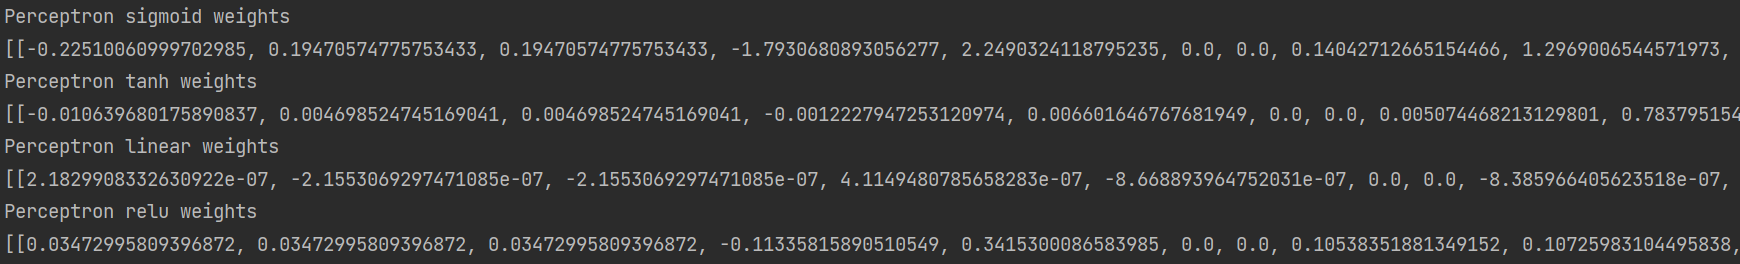
\includegraphics[width=0.8\textwidth]{img1}
\caption{Полученные веса}
\label{fig:img1}
\end{figure}

\begin{figure}[!htb]
	\centering
	
\includegraphics[width=0.8\textwidth]{img2}
\caption{Тестирование распознавания цифр}
\label{fig:img2}
\end{figure}

\begin{figure}[!htb]
	\centering
	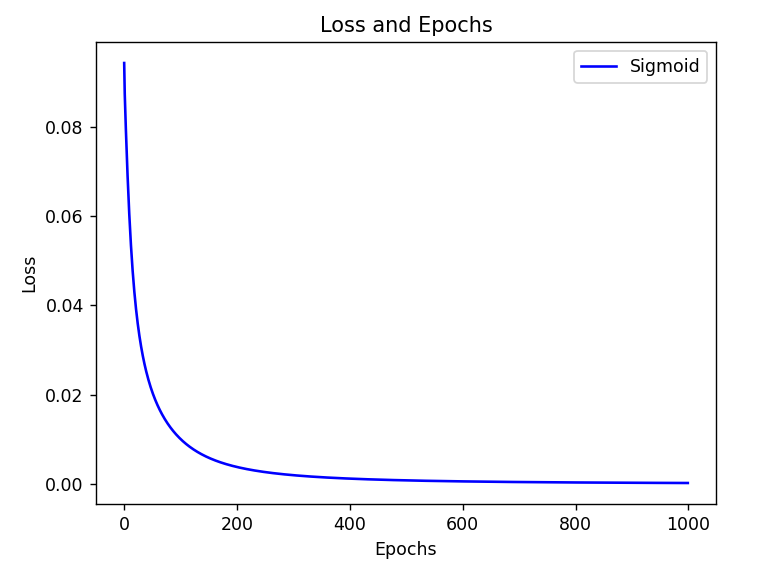
\includegraphics[width=0.8\textwidth]{img3}
\caption{Зависимость функции потерь от числа эпох}
\label{fig:img3}
\end{figure}

\begin{figure}[!htb]
	\centering
	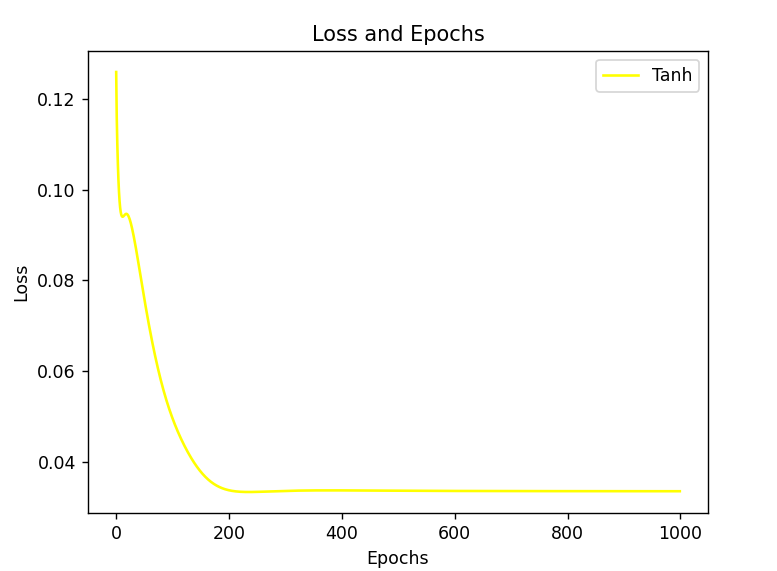
\includegraphics[width=0.8\textwidth]{img4}
\caption{Зависимость функции потерь от числа эпох}
\label{fig:img4}
\end{figure}

\begin{figure}[!htb]
	\centering
	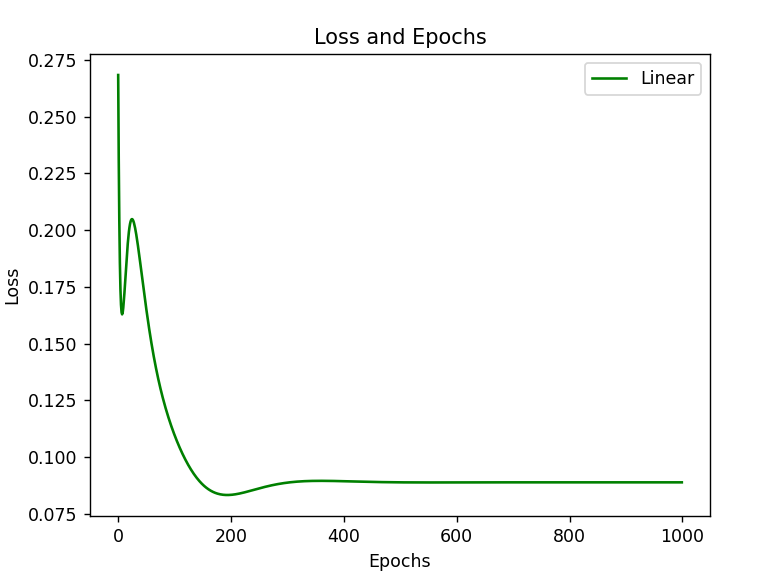
\includegraphics[width=0.8\textwidth]{img5}
\caption{Зависимость функции потерь от числа эпох}
\label{fig:img5}
\end{figure}

\begin{figure}[!htb]
	\centering
	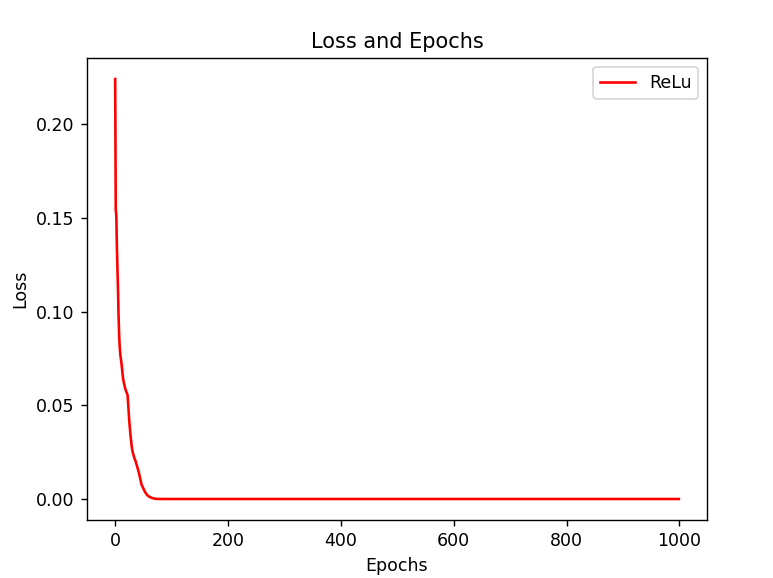
\includegraphics[width=0.8\textwidth]{img6}
\caption{Зависимость функции потерь от числа эпох}
\label{fig:img6}
\end{figure}

\section{Выводы}\label{Sect::conclusion}

В результате выполнения лабораторной работы был реализован однослойный персептрон.
\end{document}
